\pdfminorversion=4
\documentclass[aspectratio=169]{beamer}

\mode<presentation>
{
  \usetheme{default}
  \usecolortheme{default}
  \usefonttheme{default}
  \setbeamertemplate{navigation symbols}{}
  \setbeamertemplate{caption}[numbered]
  \setbeamertemplate{footline}[frame number]  % or "page number"
  \setbeamercolor{frametitle}{fg=white}
  \setbeamercolor{footline}{fg=black}
} 

\usepackage[english]{babel}
\usepackage[utf8x]{inputenc}
\usepackage{tikz}
\usepackage{courier}
\usepackage{array}
\usepackage{bold-extra}
\usepackage{minted}
\usepackage[thicklines]{cancel}
\usepackage{fancyvrb}

\xdefinecolor{dianablue}{rgb}{0.18,0.24,0.31}
\xdefinecolor{darkblue}{rgb}{0.1,0.1,0.7}
\xdefinecolor{darkgreen}{rgb}{0,0.5,0}
\xdefinecolor{darkgrey}{rgb}{0.35,0.35,0.35}
\xdefinecolor{darkorange}{rgb}{0.8,0.5,0}
\xdefinecolor{darkred}{rgb}{0.7,0,0}
\definecolor{darkgreen}{rgb}{0,0.6,0}
\definecolor{mauve}{rgb}{0.58,0,0.82}

\title[2019-04-15-irishep-aghast]{Aghast: communication among histogram implementations}
\author{Jim Pivarski}
\institute{Princeton University -- DIANA-HEP}
\date{April 15, 2019}

\usetikzlibrary{shapes.callouts}

\begin{document}

\logo{\pgfputat{\pgfxy(0.11, 7.4)}{\pgfbox[right,base]{\tikz{\filldraw[fill=dianablue, draw=none] (0 cm, 0 cm) rectangle (50 cm, 1 cm);}\mbox{\hspace{-8 cm}
\includegraphics[height=1 cm]{princeton-logo-long.png}
\includegraphics[height=1 cm]{diana-hep-logo-long.png}}}}}

\begin{frame}
  \titlepage
\end{frame}

\logo{\pgfputat{\pgfxy(0.11, 7.4)}{\pgfbox[right,base]{\tikz{\filldraw[fill=dianablue, draw=none] (0 cm, 0 cm) rectangle (50 cm, 1 cm);}\mbox{\hspace{-8 cm}
\includegraphics[height=1 cm]{princeton-logo.png}
\includegraphics[height=1 cm]{diana-hep-logo.png}}}}}

% Uncomment these lines for an automatically generated outline.
%\begin{frame}{Outline}
%  \tableofcontents
%\end{frame}

% START START START START START START START START START START START START START

\begin{frame}{Context: slide from last summer (8 table rows commented out!)}
\scriptsize
\vspace{0.35 cm}
\begin{columns}
\column{1.1\linewidth}
\renewcommand{\arraystretch}{1.2}
\begin{tabular}{c l c p{2.7 cm} p{1.5 cm} p{4.75 cm}}
pip? & name & last release & interface style & depends on & integrates with \\\hline
& \href{https://root.cern.ch/pyroot}{\textcolor{blue}{PyROOT}} & 2018 & HEP & ROOT & numpy \\
& \href{https://yoda.hepforge.org/pydoc}{\textcolor{blue}{YODA}} & 2018 & HEP & {\it compiled} & matplotlib, yaml \\
$\surd$ & \href{https://pypi.python.org/pypi/physt}{\textcolor{blue}{physt}} & 2018 & HEP + data science & numpy & pandas, xarray, dask, protobuf, matplotlib, vega (plotting), folium (maps) \\
$\surd$ & \href{https://pypi.org/project/fast-histogram}{\textcolor{blue}{fast-histogram}} & 2018 & simple (astronomy) & numpy & \\
$\surd$ & \href{https://pypi.org/project/qhist/}{\textcolor{blue}{qhist}} & 2018 & HEP & ROOT & \\
$\surd$ & \href{https://pypi.org/project/rootpy}{\textcolor{blue}{rootpy}} & 2017 & HEP & ROOT & pytables, matplotlib, stats \\
$\surd$ & \href{https://vaex.io}{\textcolor{blue}{Vaex}} (vaex.io) & 2017 & all-in-one GUI for big data, fast heatmaps & {\it many!} & Jupyter, matplotlib, HDF5, pandas, C++ \\
$\surd$ & \href{https://pypi.python.org/pypi/hdrhistogram}{\textcolor{blue}{hdrhistogram}} & 2017 & ``high dynamic range'' & {\it compiled} & Java, C++ \\
$\surd$ & \href{https://pypi.python.org/pypi/multihist}{\textcolor{blue}{multihist}} & 2017 & numpy wrapper & numpy & matplotlib \\
$\surd$ & \href{https://github.com/ibab/matplotlib-hep}{\textcolor{blue}{matplotlib-hep}} & 2016 & HEP & matplotlib & numpy, scipy \\
$\surd$ & \href{https://pypi.python.org/pypi/pyhistogram}{\textcolor{blue}{pyhistogram}} & 2014 & HEP & numpy & matplotlib, datetime \\
$\surd$ & \href{https://pypi.python.org/pypi/histogram}{\textcolor{blue}{histogram}} & 2011 & HEP & numpy & matplotlib, HDF5 \\
$\surd$ & \href{https://pypi.python.org/pypi/SimpleHist}{\textcolor{blue}{SimpleHist}} & 2011 & HEP & numpy, matplotlib & ROOT \\
$\surd$ & \href{https://pypi.org/project/paida}{\textcolor{blue}{paida}} & 2007 & HEP & & AIDA! \\
& \href{https://github.com/theodoregoetz/histogram}{\textcolor{blue}{theodoregoetz}} & never & HEP & scipy, \mbox{uncertainties} & numpy, matplotlib \\
% $\surd$ & \href{https://pypi.python.org/pypi/histogramy}{\textcolor{blue}{histogramy}} & 2013 & Numpy, Matplotlib, Scikit-Learn & & \\
% $\surd$ & \href{https://pypi.python.org/pypi/pypeaks}{\textcolor{blue}{pypeaks}} & 2014 & & & \\
% $\surd$ & \href{https://pypi.python.org/pypi/hierogram}{\textcolor{blue}{hierogram}} & 2014 & & & \\
% $\surd$ & \href{https://pypi.python.org/pypi/histo}{\textcolor{blue}{histo}} & & & & \\
% $\surd$ & \href{https://pypi.python.org/pypi/python-metrics}{\textcolor{blue}{python-metrics}} & & & & \\
% $\surd$ & \href{https://pypi.python.org/pypi/statscounter}{\textcolor{blue}{statscounter}} & 2016 & & & \\
% $\surd$ & \href{https://pypi.python.org/pypi/datagram}{\textcolor{blue}{datagram}} & & & & \\
% & \href{http://www.ifh.de/~middell/dashi/index.html}{\textcolor{blue}{dashi}} & & & & \\
\end{tabular}
\end{columns}
\end{frame}

\begin{frame}{Even more\ldots}

{\large Over the years, I've written five:}

\scriptsize
\vspace{0.25 cm}
\begin{columns}
\column{1.1\linewidth}
\renewcommand{\arraystretch}{1.2}
\begin{tabular}{c l c p{2.7 cm} p{1.5 cm} p{4.75 cm}}
pip? & name & last release & interface style & depends on & integrates with \\\hline
& \href{http://code.google.com/p/plothon}{\textcolor{blue}{Plothon}} & 2006 & HEP & ROOT & SVG \\
& \href{http://code.google.com/p/svgfig}{\textcolor{blue}{SVGFig}} & 2008 & HEP & {\it nothing!} & SVG \\
& \href{https://github.com/opendatagroup/cassius}{\textcolor{blue}{Cassius}} & 2013 & HEP + data science & numpy & SVG, Augustus (Open Data Group) \\
$\surd$ & \href{https://github.com/histogrammar}{\textcolor{blue}{Histogrammar}} & 2016 & combinational library & numpy & Spark, Julia, CUDA, \mbox{ROOT (Cling),} matplotlib, Bokeh, Vega \\
$\surd$ & \href{https://github.com/scikit-hep/histbook}{\textcolor{blue}{histbook}} & 2018 & HEP & numpy & Spark, Pandas, Vega \\
\end{tabular}
\end{columns}

\vspace{1 cm}
{\large And today, you've heard about three more:}

\begin{columns}
\column{1.1\linewidth}
\renewcommand{\arraystretch}{1.2}
\begin{tabular}{c l c p{2.7 cm} p{1.5 cm} p{4.75 cm}}
pip? & name & last release & interface style & depends on & integrates with \\\hline
$\surd$ & \href{https://gitter.im/HSF/mpl-hep}{\textcolor{blue}{mpl-hep}} & 2019 & HEP & Matplotlib & numpy, pandas \\
$\surd$ & \href{https://github.com/boostorg/histogram}{\textcolor{blue}{boost-histogram}} & 2019 & HEP & {\it compiled} & C++, numpy \\
$\surd$ & \href{https://pypi.org/project/hist/}{\textcolor{blue}{hist}} & 2019 & HEP & the above & \\
\end{tabular}
\end{columns}
\end{frame}

\begin{frame}{}
\vspace{1 cm}
\Large
\begin{center}
We're not lacking for options, but perhaps for unity.
\end{center}
\end{frame}

\begin{frame}{Tying it all together}
\large
\vspace{0.5 cm}
Moreover, these libraries are specializing:

\vspace{0.25 cm}
\begin{itemize}
\item {\bf boost-histogram} provides fast and flexible {\it filling},
\item {\bf mpl-hep} provides many {\it plotting} options.
\end{itemize}

\vspace{0.25 cm}
The {\bf hist} package will wrap that up behind a single ``\mintinline{python}{import hist}'' command, but to do so, we need to get histogram objects from one library to another.
\end{frame}

\begin{frame}{Aghast}
\large
\vspace{0.5 cm}
The {\bf aghast} library ({\bf ag}gregated, {\bf h}istogram-like {\bf st}atistics) is an {\it in-memory, serializable ontology} of histogram-like objects.

\vspace{0.75 cm}
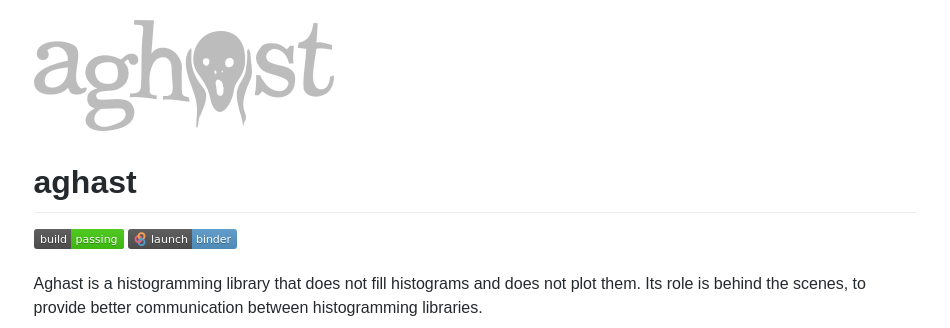
\includegraphics[width=\linewidth]{aghast-github.png}
\end{frame}

\begin{frame}{}
\vspace{1.25 cm}
\begin{description}\setlength{\itemsep}{0.5 cm}
\item[in-memory:] The purpose is to move histogram-like data from one library to another, invisibly as part of a function call. It is not primarily intended for long-term storage in files. In this respect, it is like Apache Arrow.

\item[serializable:]<2-> We use Flatbuffers as a wire protocol to move data over a network or among languages (12 supported), if necessary. Flatbuffers supports partial reading/deserialization (used in network games; must be fast).

\item[ontology:]<3-> Aghast focuses exclusively on representing the data and converting histograms into histograms. It does not fill or plot them. In this respect, it is like Predictive Model Markup Language (PMML), which neither trains nor scores machine learning models.
\end{description}
\end{frame}

\begin{frame}[fragile]{What does it look like?}
\small
\begin{minted}{python}
>>> import numpy, aghast
>>> h_numpy = numpy.histogram(numpy.random.normal(0, 1, 100000),
...                           bins=20, range=(-5, 5))
>>> aghast.from_numpy(h_numpy).dump()
\end{minted}

\scriptsize
\begin{verbatim}
Histogram(
  axis=[
    Axis(binning=RegularBinning(num=20, interval=RealInterval(low=-5.0, high=5.0)))
  ],
  counts=
    UnweightedCounts(
      counts=
        InterpretedInlineInt64Buffer(
          buffer=
              [    2     5    21   107   477  1696  4378  9146 15084 19273 18933 14960
                9216  4425  1648   480   122    23     4     0])))
\end{verbatim}

\vspace{0.25 cm}
\uncover<2->{\textcolor{darkblue}{\large Very formal class hierarchy, long names $\to$ not for end-users!}}
\end{frame}

\begin{frame}[fragile]{What does it look like?}
\small
\begin{minted}{python}
>>> import ROOT, aghast
>>> h_root = ROOT.TH1F("name", "title", 20, -5, 5)
>>> h_root.FillRandom("gaus", 100000)
>>> aghast.from_root(h_root).dump()
\end{minted}

\uncover<2->{(The ROOT histogram has {\tt moments} to preserve unbinned mean and standard deviation.)}

\tiny
\begin{verbatim}
Histogram(
  axis=[
    Axis(
      binning=
        RegularBinning(
          num=20,
          interval=RealInterval(low=-5.0, high=5.0),
          overflow=RealOverflow(loc_underflow=BinLocation.below1, loc_overflow=BinLocation.above1)),
      statistics=[
        Statistics(
          moments=[
            Moments(sumwxn=InterpretedInlineInt64Buffer(buffer=[100000]), n=0),
            Moments(sumwxn=InterpretedInlineFloat64Buffer(buffer=[100000]), n=0, weightpower=1),
            Moments(sumwxn=InterpretedInlineFloat64Buffer(buffer=[100000]), n=0, weightpower=2),
            Moments(sumwxn=InterpretedInlineFloat64Buffer(buffer=[-102.751]), n=1, weightpower=1),
            Moments(sumwxn=InterpretedInlineFloat64Buffer(buffer=[104061]), n=2, weightpower=1)
          ])
      ])
  ],
  counts=
    UnweightedCounts(
      counts=
        InterpretedInlineBuffer(
          buffer=
              [0.0000e+00 0.0000e+00 4.0000e+00 1.8000e+01 1.0000e+02 4.7900e+02
               1.6950e+03 4.3380e+03 9.2950e+03 1.4974e+04 1.9195e+04 1.9289e+04
               1.4781e+04 9.1450e+03 4.3850e+03 1.6680e+03 4.9200e+02 1.1600e+02
               2.3000e+01 3.0000e+00 0.0000e+00 0.0000e+00],
          dtype=Interpretation.float32)),
  title='title')
\end{verbatim}
\end{frame}

\begin{frame}[fragile]{What does it look like?}
\small
\begin{minted}{python}
>>> aghast.to_numpy(aghast.from_root(h_root))
\end{minted}

\scriptsize
\begin{verbatim}
(array([0.0000e+00, 0.0000e+00, 4.0000e+00, 1.8000e+01, 1.0000e+02,
       4.7900e+02, 1.6950e+03, 4.3380e+03, 9.2950e+03, 1.4974e+04,
       1.9195e+04, 1.9289e+04, 1.4781e+04, 9.1450e+03, 4.3850e+03,
       1.6680e+03, 4.9200e+02, 1.1600e+02, 2.3000e+01, 3.0000e+00,
       0.0000e+00, 0.0000e+00], dtype=float32),
 array([-inf, -5. , -4.5, -4. , -3.5, -3. , -2.5, -2. , -1.5, -1. , -0.5,
        0. ,  0.5,  1. ,  1.5,  2. ,  2.5,  3. ,  3.5,  4. ,  4.5,  5. ,
        inf]))
\end{verbatim}

\uncover<2->{\large Even though Numpy doesn't have a concept of regularly spaced bins or overflow bins, we can shoehorn the ROOT histogram into this form.}
\end{frame}

\begin{frame}[fragile]{What does it look like?}
\vspace{0.5 cm}
\small
\begin{minted}{python}
>>> aghast.to_root(aghast.from_numpy(h_numpy), "name").Draw()
\end{minted}

\begin{center}
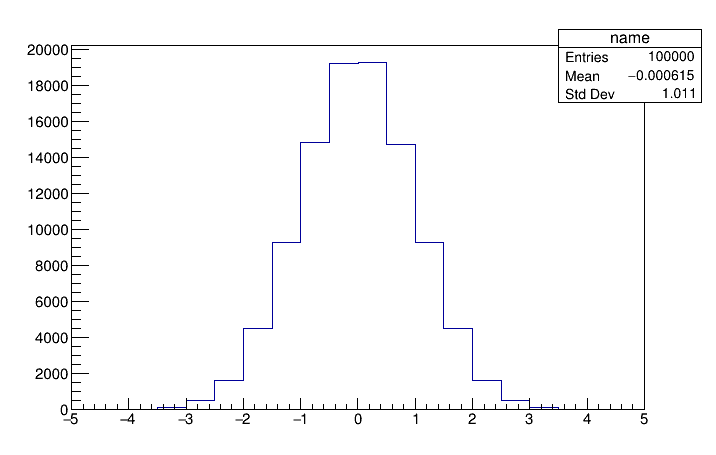
\includegraphics[width=0.65\linewidth]{c1.png}
\end{center}
\end{frame}

\begin{frame}[fragile]{What does it look like?}
\vspace{0.5 cm}
\small
\begin{minted}{python}
>>> aghast.to_pandas(aghast.from_root(h_root))
\end{minted}

\tiny
\begin{verbatim}
              unweighted
[-inf, -5.0)         0.0
[-5.0, -4.5)         0.0
[-4.5, -4.0)         4.0
[-4.0, -3.5)        18.0
[-3.5, -3.0)       100.0
[-3.0, -2.5)       479.0
[-2.5, -2.0)      1695.0
[-2.0, -1.5)      4338.0
[-1.5, -1.0)      9295.0
[-1.0, -0.5)     14974.0
[-0.5, 0.0)      19195.0
[0.0, 0.5)       19289.0
[0.5, 1.0)       14781.0
[1.0, 1.5)        9145.0
[1.5, 2.0)        4385.0
[2.0, 2.5)        1668.0
[2.5, 3.0)         492.0
[3.0, 3.5)         116.0
[3.5, 4.0)          23.0
[4.0, 4.5)           3.0
[4.5, 5.0)           0.0
[5.0, inf)           0.0
\end{verbatim}
\end{frame}

%% >>> tmessage = ROOT.TMessage()
%% >>> tmessage.WriteObject(h_root)
%% >>> tmessage.Length()
%% 642
%% >>> len(aghast.from_root(h_root).tobuffer())
%% 544

\begin{frame}{Common way of describing features in all histogram libraries}
\vspace{0.25 cm}
\scriptsize
\begin{columns}[t]
\column{0.33\linewidth}
\begin{itemize}
  \item \href{https://github.com/scikit-hep/aghast/blob/master/specification.adoc\#collection}{\textcolor{blue}{Collection}}
  \item \href{https://github.com/scikit-hep/aghast/blob/master/specification.adoc\#histogram}{\textcolor{blue}{Histogram}}
  \item \href{https://github.com/scikit-hep/aghast/blob/master/specification.adoc\#axis}{\textcolor{blue}{Axis}}
  \item \href{https://github.com/scikit-hep/aghast/blob/master/specification.adoc\#integerbinning}{\textcolor{blue}{IntegerBinning}}
  \item \href{https://github.com/scikit-hep/aghast/blob/master/specification.adoc\#regularbinning}{\textcolor{blue}{RegularBinning}}
  \item \href{https://github.com/scikit-hep/aghast/blob/master/specification.adoc\#realinterval}{\textcolor{blue}{RealInterval}}
  \item \href{https://github.com/scikit-hep/aghast/blob/master/specification.adoc\#realoverflow}{\textcolor{blue}{RealOverflow}}
  \item \href{https://github.com/scikit-hep/aghast/blob/master/specification.adoc\#hexagonalbinning}{\textcolor{blue}{HexagonalBinning}}
  \item \href{https://github.com/scikit-hep/aghast/blob/master/specification.adoc\#edgesbinning}{\textcolor{blue}{EdgesBinning}}
  \item \href{https://github.com/scikit-hep/aghast/blob/master/specification.adoc\#irregularbinning}{\textcolor{blue}{IrregularBinning}}
  \item \href{https://github.com/scikit-hep/aghast/blob/master/specification.adoc\#categorybinning}{\textcolor{blue}{CategoryBinning}}
  \item \href{https://github.com/scikit-hep/aghast/blob/master/specification.adoc\#sparseregularbinning}{\textcolor{blue}{SparseRegularBinning}}
  \item \href{https://github.com/scikit-hep/aghast/blob/master/specification.adoc\#fractionbinning}{\textcolor{blue}{FractionBinning}}
  \item \href{https://github.com/scikit-hep/aghast/blob/master/specification.adoc\#predicatebinning}{\textcolor{blue}{PredicateBinning}}
  \item \href{https://github.com/scikit-hep/aghast/blob/master/specification.adoc\#variationbinning}{\textcolor{blue}{VariationBinning}}
\end{itemize}
\column{0.33\linewidth}
\begin{itemize}
  \item \href{https://github.com/scikit-hep/aghast/blob/master/specification.adoc\#variation}{\textcolor{blue}{Variation}}
  \item \href{https://github.com/scikit-hep/aghast/blob/master/specification.adoc\#assignment}{\textcolor{blue}{Assignment}}
  \item \href{https://github.com/scikit-hep/aghast/blob/master/specification.adoc\#unweightedcounts}{\textcolor{blue}{UnweightedCounts}}
  \item \href{https://github.com/scikit-hep/aghast/blob/master/specification.adoc\#weightedcounts}{\textcolor{blue}{WeightedCounts}}
  \item \href{https://github.com/scikit-hep/aghast/blob/master/specification.adoc\#interpretedinlinebuffer}{\textcolor{blue}{InterpretedInlineBuffer}}
  \item \href{https://github.com/scikit-hep/aghast/blob/master/specification.adoc\#interpretedinlineint64buffer}{\textcolor{blue}{InterpretedInlineInt64Buffer}}
  \item \href{https://github.com/scikit-hep/aghast/blob/master/specification.adoc\#interpretedinlinefloat64buffer}{\textcolor{blue}{InterpretedInlineFloat64Buffer}}
  \item \href{https://github.com/scikit-hep/aghast/blob/master/specification.adoc\#interpretedexternalbuffer}{\textcolor{blue}{InterpretedExternalBuffer}}
  \item \href{https://github.com/scikit-hep/aghast/blob/master/specification.adoc\#profile}{\textcolor{blue}{Profile}}
  \item \href{https://github.com/scikit-hep/aghast/blob/master/specification.adoc\#statistics}{\textcolor{blue}{Statistics}}
  \item \href{https://github.com/scikit-hep/aghast/blob/master/specification.adoc\#moments}{\textcolor{blue}{Moments}}
  \item \href{https://github.com/scikit-hep/aghast/blob/master/specification.adoc\#quantiles}{\textcolor{blue}{Quantiles}}
  \item \href{https://github.com/scikit-hep/aghast/blob/master/specification.adoc\#modes}{\textcolor{blue}{Modes}}
  \item \href{https://github.com/scikit-hep/aghast/blob/master/specification.adoc\#extremes}{\textcolor{blue}{Extremes}}
  \item \href{https://github.com/scikit-hep/aghast/blob/master/specification.adoc\#statisticfilter}{\textcolor{blue}{StatisticFilter}}
\end{itemize}
\column{0.33\linewidth}
\begin{itemize}
  \item \href{https://github.com/scikit-hep/aghast/blob/master/specification.adoc\#covariance}{\textcolor{blue}{Covariance}}
  \item \href{https://github.com/scikit-hep/aghast/blob/master/specification.adoc\#parameterizedfunction}{\textcolor{blue}{ParameterizedFunction}}
  \item \href{https://github.com/scikit-hep/aghast/blob/master/specification.adoc\#parameter}{\textcolor{blue}{Parameter}}
  \item \href{https://github.com/scikit-hep/aghast/blob/master/specification.adoc\#evaluatedfunction}{\textcolor{blue}{EvaluatedFunction}}
  \item \href{https://github.com/scikit-hep/aghast/blob/master/specification.adoc\#binnedevaluatedfunction}{\textcolor{blue}{BinnedEvaluatedFunction}}
  \item \href{https://github.com/scikit-hep/aghast/blob/master/specification.adoc\#ntuple}{\textcolor{blue}{Ntuple}}
  \item \href{https://github.com/scikit-hep/aghast/blob/master/specification.adoc\#column}{\textcolor{blue}{Column}}
  \item \href{https://github.com/scikit-hep/aghast/blob/master/specification.adoc\#ntupleinstance}{\textcolor{blue}{NtupleInstance}}
  \item \href{https://github.com/scikit-hep/aghast/blob/master/specification.adoc\#chunk}{\textcolor{blue}{Chunk}}
  \item \href{https://github.com/scikit-hep/aghast/blob/master/specification.adoc\#columnchunk}{\textcolor{blue}{ColumnChunk}}
  \item \href{https://github.com/scikit-hep/aghast/blob/master/specification.adoc\#page}{\textcolor{blue}{Page}}
  \item \href{https://github.com/scikit-hep/aghast/blob/master/specification.adoc\#rawinlinebuffer}{\textcolor{blue}{RawInlineBuffer}}
  \item \href{https://github.com/scikit-hep/aghast/blob/master/specification.adoc\#rawexternalbuffer}{\textcolor{blue}{RawExternalBuffer}}
  \item \href{https://github.com/scikit-hep/aghast/blob/master/specification.adoc\#metadata}{\textcolor{blue}{Metadata}}
  \item \href{https://github.com/scikit-hep/aghast/blob/master/specification.adoc\#decoration}{\textcolor{blue}{Decoration}}
\end{itemize}
\end{columns}
\end{frame}

\begin{frame}{Common way of describing features in all histogram libraries}
\vspace{0.5 cm}
\begin{itemize}
\item Only one {\bf Histogram} type; it's n-dimensional and slicable like a Numpy array.
\item Regular/irregular/string-labeled/sparse axis types are all {\bf Binnings} (and they become an index or multi-index in Pandas).
\item Efficiency plots are plots that have a {\bf FractionBinning} in some axis.
\item {\bf Collections} of plots representing the same observables with different cuts share a {\bf PredicateBinning}.
\item {\bf Collections} of plots representing different systematic variations share a {\bf VariationBinning}.
\item An {\bf Axis} may also have {\bf Moments} and {\bf Correlations}.
\item {\bf Profile} plots are those that have binned {\bf Moments}. Many {\bf Profiles} can share the same binning (and they become columns in Pandas).
\item {\bf Functions} may be attached to {\bf Histograms} or may be unattached in {\bf Collections}.
\item {\bf Collections} may also contain simple {\bf Ntuples} for unbinned fitting.
\end{itemize}
\end{frame}


\end{document}
